\documentclass[]{revtex4}\usepackage[]{graphicx}\usepackage[]{color}
%% maxwidth is the original width if it is less than linewidth
%% otherwise use linewidth (to make sure the graphics do not exceed the margin)
\makeatletter
\def\maxwidth{ %
  \ifdim\Gin@nat@width>\linewidth
    \linewidth
  \else
    \Gin@nat@width
  \fi
}
\makeatother

\definecolor{fgcolor}{rgb}{0.345, 0.345, 0.345}
\newcommand{\hlnum}[1]{\textcolor[rgb]{0.686,0.059,0.569}{#1}}%
\newcommand{\hlstr}[1]{\textcolor[rgb]{0.192,0.494,0.8}{#1}}%
\newcommand{\hlcom}[1]{\textcolor[rgb]{0.678,0.584,0.686}{\textit{#1}}}%
\newcommand{\hlopt}[1]{\textcolor[rgb]{0,0,0}{#1}}%
\newcommand{\hlstd}[1]{\textcolor[rgb]{0.345,0.345,0.345}{#1}}%
\newcommand{\hlkwa}[1]{\textcolor[rgb]{0.161,0.373,0.58}{\textbf{#1}}}%
\newcommand{\hlkwb}[1]{\textcolor[rgb]{0.69,0.353,0.396}{#1}}%
\newcommand{\hlkwc}[1]{\textcolor[rgb]{0.333,0.667,0.333}{#1}}%
\newcommand{\hlkwd}[1]{\textcolor[rgb]{0.737,0.353,0.396}{\textbf{#1}}}%

\usepackage{framed}
\makeatletter
\newenvironment{kframe}{%
 \def\at@end@of@kframe{}%
 \ifinner\ifhmode%
  \def\at@end@of@kframe{\end{minipage}}%
  \begin{minipage}{\columnwidth}%
 \fi\fi%
 \def\FrameCommand##1{\hskip\@totalleftmargin \hskip-\fboxsep
 \colorbox{shadecolor}{##1}\hskip-\fboxsep
     % There is no \\@totalrightmargin, so:
     \hskip-\linewidth \hskip-\@totalleftmargin \hskip\columnwidth}%
 \MakeFramed {\advance\hsize-\width
   \@totalleftmargin\z@ \linewidth\hsize
   \@setminipage}}%
 {\par\unskip\endMakeFramed%
 \at@end@of@kframe}
\makeatother

\definecolor{shadecolor}{rgb}{.97, .97, .97}
\definecolor{messagecolor}{rgb}{0, 0, 0}
\definecolor{warningcolor}{rgb}{1, 0, 1}
\definecolor{errorcolor}{rgb}{1, 0, 0}
\newenvironment{knitrout}{}{} % an empty environment to be redefined in TeX

\usepackage{alltt} %twocolumn revtex4
\usepackage[T1]{fontenc}
\usepackage{lmodern}
\usepackage{booktabs}
\usepackage{graphicx,subfig}
\IfFileExists{upquote.sty}{\usepackage{upquote}}{}
\begin{document}

\title{Simulated and UK tree clustered by UCSD soft. - March 2016}
\author{S. Le Vu}
%\affiliation{ICL}
\date{\today}

\maketitle





\section{Intro}
\begin{itemize}
\item "Time-based" distances from \emph{simulated} coalescent tree are converted to substitutions per site distances with a constant rate from the litterature
\item Then matrices of distances are converted in edge lists of pairwise distances with header ID1, ID2, distance as needed by UCSD software \texttt{hivclustering}
\item Edge lists are inputed in the \texttt{hivnetworkcsv} function which returns lists of cluster assignements
\end{itemize}


\begin{figure}
     \centering
     \subfloat[][Simulation]{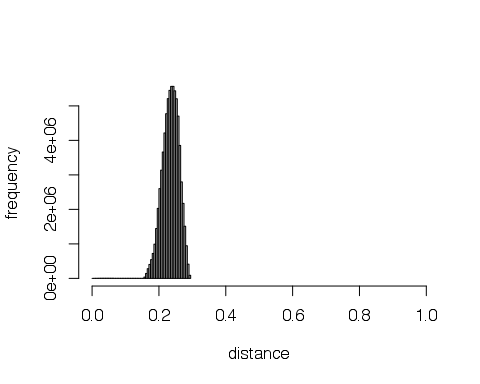
\includegraphics[scale=0.5]{figure/simtree_dist.png}}
     \subfloat[][UK]{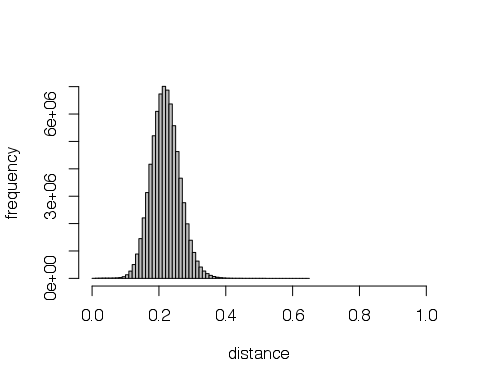
\includegraphics[scale=0.5]{figure/uktree_dist.png}}
     \caption{Distances (subst/site)}
\end{figure}

%' << load sim, echo = FALSE, include = T >>=
%' 
%' @
%' 
%' \section{UCSD hivclustering}
%' Read saved results from UCSD \textsf{hivclustering}
%' << read >>=
%' @
%' 
%' 
%' To construct clusters, threshold were determined by quantiles of distances (0.05\%, 0.1\%, 1\% and 10\%). For simulated and UK trees
%' << quantiles >>=
%' @
%' 
%' Number of clusters and stats for simulated and UK trees (cluster size 1 does not exist in these outputs)
%' << desc >>=
%' @
%' 
%' Plots of log(size) for UK and simulated clusters
%' << plot log-log >>=
%' @
%' 
%' QQ plots UK vs simulated, untransformed and log-log
%' << QQ plot >>=
%' @
%' 
%' \section{Associations}
%' After merging with co-variates allocated from demes states contained in tree, non-clustering individuals are assigned a cluster size of 1. 
%' << data >>=
%' @
%' 
%' The proportion of individuals into clusters and stats for "size of cluster for each individuals"
%' <<demo, echo = FALSE, include = FALSE>>=
%' @
%' 
%' << proportion >>=
%' @
%' 
%' << merge, echo = FALSE >>=
%' @
%' 
%' \section{Naive regressions on simulation}
%' 
%' Linear
%' << sim linear >>=
%' 
%' @
%' 
%' Logistic
%' << sim logistic >>=
%' 
%' @
%' 
%' \section{Regressions on down-sampled simulation}
%' To sort out the dependency between individuals from same cluster
%' \begin{enumerate}
%' \item "downsample" to make analysis of each cluster size explained by mean of each co-variate (from here, only clusters from lower and higher threshold represented)
%' 
%' << downsample >>=
%' @
%' 
%' 
%' \item plot the distribution of covariates by cluster size
%' 
%' << lattice >>=
%' @
%' 
%' 
%' \end{enumerate}
%' 
%' \section{On real UK data}
%' Same process ...
%' <<multivariate, echo=FALSE>>=
%' @
%' 
%' Proportion in and out clusters
%' << proportion UK>>=
%' @
%' 
%' <<merge UK, echo=FALSE>>=
%' 
%' @
%' 
%' Naive regressions
%' <<linear UK>>=
%' @
%' 
%' <<logistic UK>>=
%' @
%' 
%' Down-sampled regressions
%' <<downsample UK>>=
%' @
%' 
%' <<lattice UK>>=
%' @


\end{document}
